% !TEX program = pdflatex
%%%%%%%%%%%%%%%%%%%%%%%%%%%%%%%%%%%%%%%%%
% Structured General Purpose Assignment
% LaTeX Template
%
% This template has been downloaded from:
% http://www.latextemplates.com
%
% Original author:
% Ted Pavlic (http://www.tedpavlic.com)
%
% Note:
% The \lipsum[#] commands throughout this template generate dummy text
% to fill the template out. These commands should all be removed when
% writing assignment content.
%
%%%%%%%%%%%%%%%%%%%%%%%%%%%%%%%%%%%%%%%%%

%----------------------------------------------------------------------------------------
%	PACKAGES AND OTHER DOCUMENT CONFIGURATIONS
%----------------------------------------------------------------------------------------

\documentclass{article}

\usepackage{fancyhdr} % Required for custom headers
\usepackage{lastpage} % Required to determine the last page for the footer
\usepackage{extramarks} % Required for headers and footers
\usepackage{graphicx} % Required to insert images
\usepackage{subcaption}
\usepackage{lipsum} % Used for inserting dummy 'Lorem ipsum' text into the template

\usepackage[utf8]{inputenc}
\usepackage[ngerman,english]{babel}
\usepackage[T1]{fontenc}
\usepackage{breakurl}
\usepackage[hyphens]{url}
\usepackage{color}
\usepackage{float}
\usepackage{hyperref}
\usepackage{tabularx}
\usepackage{enumitem}
\usepackage{color, colortbl}
\usepackage[super]{nth}
\usepackage{epigraph}
\usepackage{titlesec}

\usepackage[
	backend=biber,
	style=numeric-comp,
	natbib=true,
	url=false,
	doi=false,
	eprint=false,
	sorting=none,
	isbn=false]
	{biblatex}

\bibliography{references}

\addto\captionsenglish{
  \renewcommand{\contentsname}%
    {Table of Contents}%
}

% Margins
\topmargin=-0.45in
\evensidemargin=0in
\oddsidemargin=0in
\textwidth=6.5in
\textheight=9.0in
\headsep=0.25in

\linespread{1.1} % Line spacing
% Set up the header and footer
\pagestyle{fancy}
\lhead{} % Top left header
\chead{Advanced Topics of Software Engineering Summary} % Top center header
\rhead{\firstxmark} % Top right header
\lfoot{\lastxmark} % Bottom left footer
\cfoot{} % Bottom center footer
\rfoot{Page\ \thepage\ of\ \pageref{LastPage}} % Bottom right footer
\renewcommand\headrulewidth{0.4pt} % Size of the header rule
\renewcommand\footrulewidth{0.4pt} % Size of the footer rule

\setlength\parindent{0pt} % Removes all indentation from paragraphs

% use paragraph as "subsubsubsection"
\titleformat{\paragraph}
{\normalfont\normalsize\bfseries}{\theparagraph}{1em}{}
\titlespacing*{\paragraph}
{0pt}{3.25ex plus 1ex minus .2ex}{1.5ex plus .2ex}

\hypersetup{	% Remove red boxes around links in table of contents
	pdfborder={0 0 0}
}


% Defining chapquote environment
\makeatletter
\newenvironment{chapquote}[2][2em]
{\setlength{\@tempdima}{#1}%
    \def\chapquote@author{#2}%
    \parshape 1 \@tempdima \dimexpr\textwidth-2\@tempdima\relax%
    \itshape}
{\par\normalfont\hfill--\ \chapquote@author\hspace*{\@tempdima}\par\bigskip}
\makeatother

\begin{document}
\setcounter{tocdepth}{3}

%----------------------------------------------------------------------------------------
% TITLE PAGE
%----------------------------------------------------------------------------------------
\pagenumbering{gobble}
% \maketitle
\begin{titlepage}
  \centering
\includegraphics[width=5cm]{tumlogo}

  \vspace{2.5cm}
  \Huge{Advanced Topics of Software Engineering} \\
  \vspace{0.1in}\huge{Lecture Summary}\\

  \Large
  \vspace{1.5cm}
  \begin{tabularx}{9cm}{r l}
    Authors: Benedikt Schlagberger
  \end{tabularx}

  \vspace{1.5cm}
  Feel free to contribute at
  \hyperlink{https://github.com/acidg/ase_summary}{https://github.com/acidg/ase\_summary}

  \vfill
  \textbf{2016-02-22} \\
  \vspace{0.3in}\normalsize{Advanced Topics of Software Engineering}\\
  \vspace{0.03in}\normalsize{\textsc{Technische Universität München}}\\
  \vspace{1cm}

\end{titlepage}
%----------------------------------------------------------------------------------------
\newpage
\section*{Disclaimer}
This is a summary of the lecture Advanced Topics of Software Engineering hold by Prof. Dr. Alexander Pretschner at TUM in the winter term 2016/2017.
The authors do not guarantee the correctness or completeness of the provided information.

\newpage
\thispagestyle{empty}
\tableofcontents

\newpage
\pagenumbering{arabic}

\section{Introduction}
This lecture is about understanding how to build complex (software) systems, which trade-offs there are between quality and the architecture and how to efficiently deliver the developed software to the stakeholders.
For that, different modeling techniques, system analysis and design with quality trade-offs, patterns, guidelines and best-practices are taught and tools for system configuration, integration and deployment are explained.

The lecture is separated into 4 chapters:
\begin{enumerate}
    \item Context of Software Engineering
        \subitem {\small Introduction, characteristics of software systems in different domains, case studies and factors affecting the design of a software system}
    \item From (quality) requirements to system design
        \subitem {\small Software architecture, libraries and frameworks, antipatterns, model-driven engineering, software product line engineering, safety and security, testability}
    \item Software architectures and their trade-offs
        \subitem {\small Distributed systems and middleware, database-, message-, object-, component- and service-oriented architectures}
    \item From source code to physical deployment
        \subitem {\small Historical perspective, version control, continuous integration and deployment, virtual machines and containers, software architectures for the cloud}
\end{enumerate}

\subsection{Characteristics of Software Systems}
Software eningeering can be separated into the technical \& management and the application domain.
The technical \& management domain contain the software system with limiting factors.
First, there are different targets defining those borders: Beside the technical infrastructure which is defining the system's size, cost, quality, time and the functionality target are set limits.
Those factors again are influenced by the process (high control) used to develop the system and the constraints (limited control: money, stakeholders, environmental influences, ...) limiting the resources available during development of the system.

The application domain is influencing the functionality target (e.g. needed functionality, available inputs and outputs, ...) and the constrains (money, management, ...) in the technical \& management domain.

The application domain can be divided into 
\begin{itemize}[topsep=5pt, itemsep=0pt]
    \item \textbf{Embedded} systems \textit{electronic devices, transportation, intelligent homes, ...}
    \item \textbf{Information} systems \textit{logistics, marketing tools, management tools, ...}
    \item \textbf{Cyberphysical} systems (connects embedded and information system) \textit{networks, reading sensors and putting out information, ...}
    \item (\textbf{Scientific software} systems \textit{not covered})
\end{itemize}



\subsection{Definition: Software Engineering}
\begin{chapquote}{"Perspectives on software engineering." Zelkowitz. (1978)}
    Study of the principles and methodologies for developing and maintaining software systems.
\end{chapquote}
\begin{chapquote}{"Software engineering: methods and management." Pfleeger. (1990)}
    Methods and techniques to develop and maintain quality software to solve
    problems.
\end{chapquote}
\begin{chapquote}{"Software engineering." Sommerville. (2010)}
    Software engineering is an engineering discipline which is concerned with all
    aspects of software production.
\end{chapquote}

Software Engineering is a collection of \textbf{techniques}, \textbf{methodologies} and \textbf{tools} that help with the production of a \textbf{\textit{high quality}} software system with a \textbf{\textit{given budget}} before a \textbf{\textit{given deadline}} while \textbf{\textit{change occurs}}.
It is essentially a problem solving activity for which first the problem is analyzed and broken down into pieces to understand the nature of the problem and later is synthesized into a large structure using \textbf{techniques}, \textbf{methodologies} and \textbf{tools}.

\begin{itemize}
    \item \textbf{Techniques} Formal procedures for producing results using some well-defined notation
    \item \textbf{Methodologies} Collection of techniques applied across software development and unified by a philosophical approach
    \item \textbf{Tools}
        \begin{itemize}[topsep=-5pt, itemsep=0pt]
            \item Instruments or automated systems to accomplish a technique
            \item Integrated Development Environment (IDE)
            \item Computer Aided Software Engineering (CASE)
        \end{itemize}
\end{itemize}

\begin{figure}[h]
    \centering
    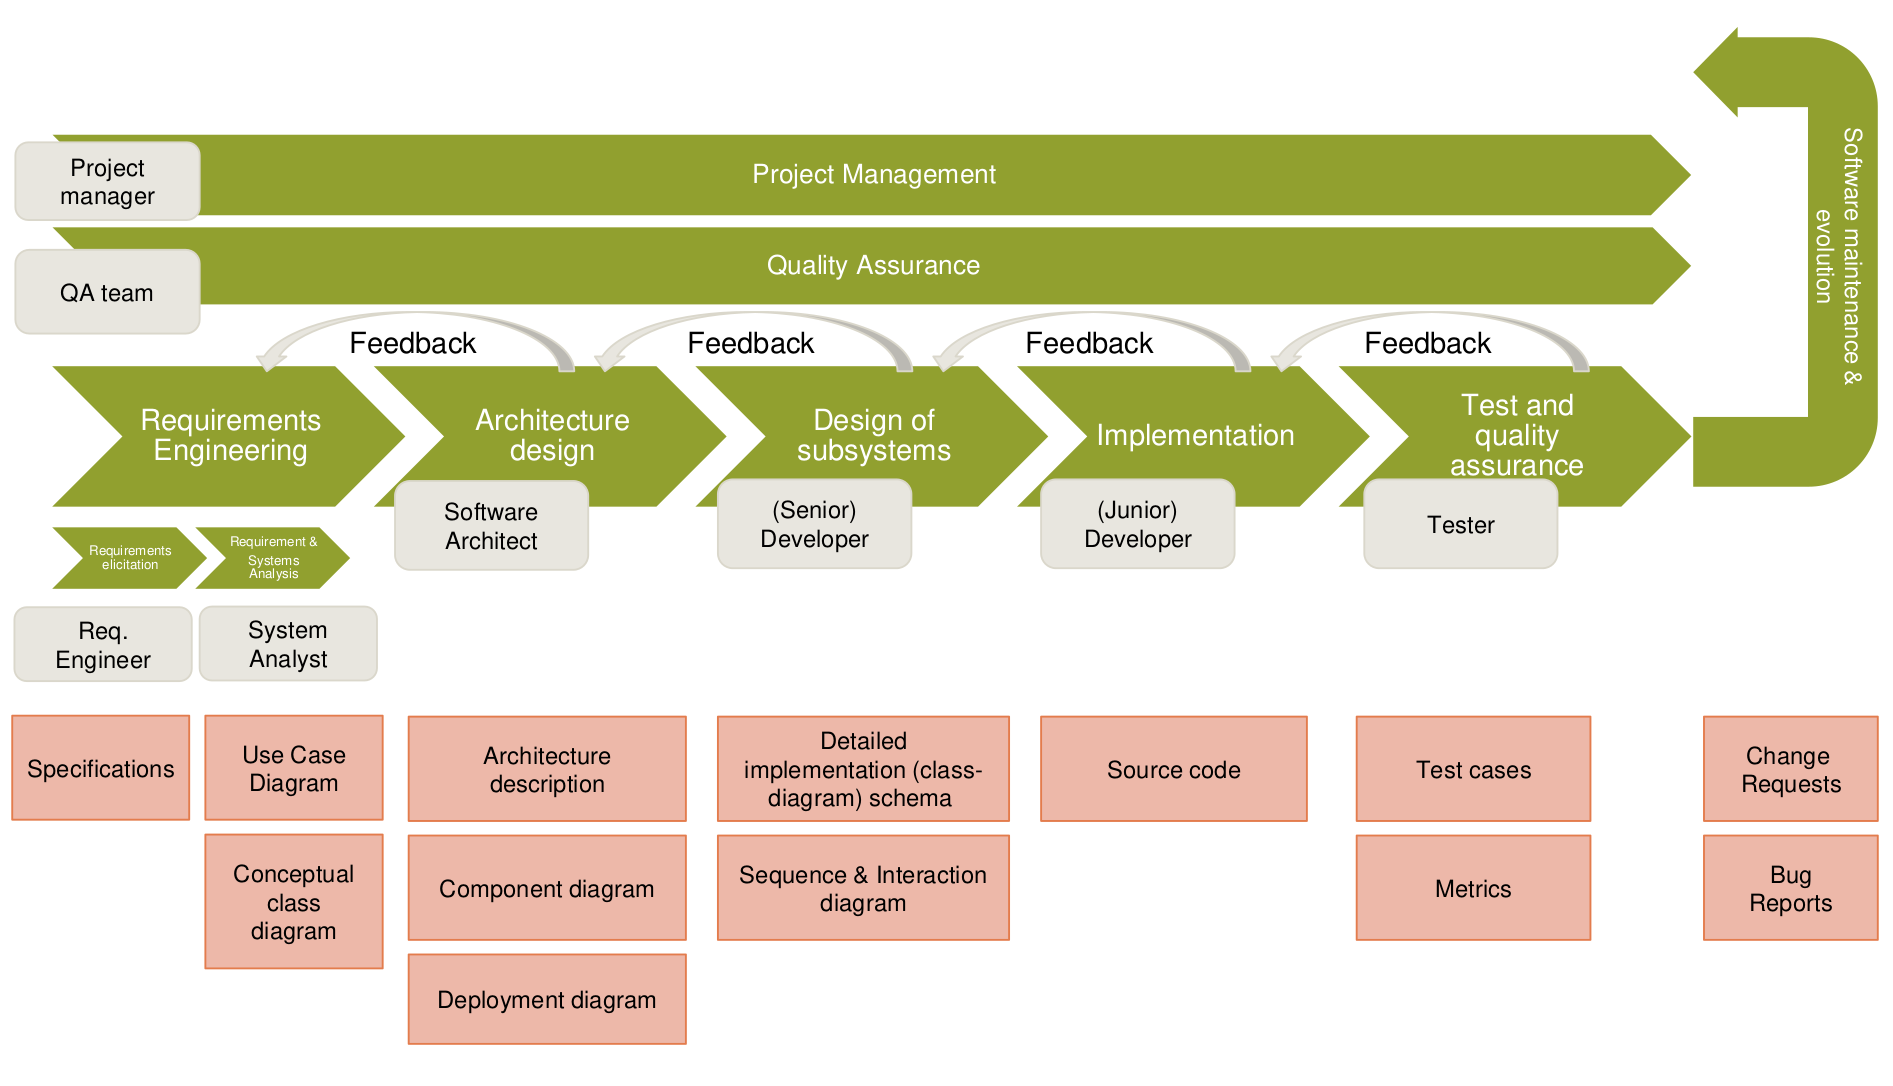
\includegraphics[width=\linewidth]{images/se_activities_roles_artifacts.png}
    \caption{Software Engineering Activities, Roles and Artifacts}\label{fig:se_activities_roles_artifacts}
\end{figure}

\subsubsection{The Process Model}
A process model describes the systematic, engineering-based, and quantifiable approach to solve a particular class of repeatable problems.
It is an abstract representation of the software process.

Some examples are:
\begin{itemize}
    \item Waterfall model \textit{\textbf{phase oriented}, classical/conventional model, inflexible (\textbf{sequential} procedure enforced), risky (errors found late and expensive)}
    \item V-Model \textit{Iterative model, \textbf{phase oriented, multiple pass}, loosely based on Waterfall, project definition then project test and integration}
    \item Unified Process \textit{Incremental model, development in expansion stages, 4 phases:Inception, Elaboration, Construction, Transition}
\end{itemize}

% TODO maybe more about unified process?

\paragraph{Agile development}
Focus on software to solve customer's problem. Less buerocratic approach. Example: Scrum (daily and stand up meetings, sprints (solving tasks from backlog))
\begin{itemize}
    \item \textbf{Individuals and interactions} over processes and tools
    \item \textbf{Working software} over comprehensive documentation
    \item \textbf{Customer collaboration} over contract negotiation
    \item \textbf{Responding to change} over following a plan
\end{itemize}

\subsubsection{Artifacts in Software Engineering}
The following lists artifacts generated during different stages of the software development process.
\paragraph{Requirements Engineering} Feasibility Report, System Models, User and System Requirements, Requirements Document
\paragraph{Software Design} System Architecture, Database Specification, Interface Specification, Component Specification
\paragraph{Testing} Acceptance Test Plan, System Integration Test Plan, Sub-System Integration Test Plan

\subsubsection{Software Quality}
\begin{chapquote}{loosely based on Balzert}
    Software quality refers to the entire characteristics of a software product that
    influence its ability to fulfill specified requirements and stakeholder expectations.
\end{chapquote}
\begin{chapquote}{"ISO 9000 - Quality management" http://www.iso.org/iso/iso\_9000}
    (Software) Quality is the degree to which a set of inherent characteristics fulfills requirements, meaning needs or expectations that are stated, generally implied or obligatory.
\end{chapquote}

Quality is a key factor for the product's success and customer's satisfaction.
In many cases quality demands are fixed (e.g. laws, contracts, ...).
Quality is tightly coupled with Non-functional requirements (NFR), but they are in general not the same.
In the lecture, quality is the sum of the process quality and the product quality (NFRs). It essentially is more than just NFRs.

Increased quality has trade-offs and can either support other quality aspects (e.g. maintainability vs. portability), or negatively influence them (security vs. efficiency).

To maximize the quality of a system, quality aspects and its interdependencies have to be assessed and balanced and prioritized in a way, where negative trade-offs are small.
Those trade-offs and prioritizations are highly situation and project dependent.

The quality of the developed product is influenced by the quality of the production process, but the correlation is complex (see \autoref{fig:se_process_vs_quality}), since software development is a creative, rather than a mechanical process.
Measuring the quality of software is difficult (e.g. measuring maintainability needs a long time).

\begin{figure}[h]
    \centering
    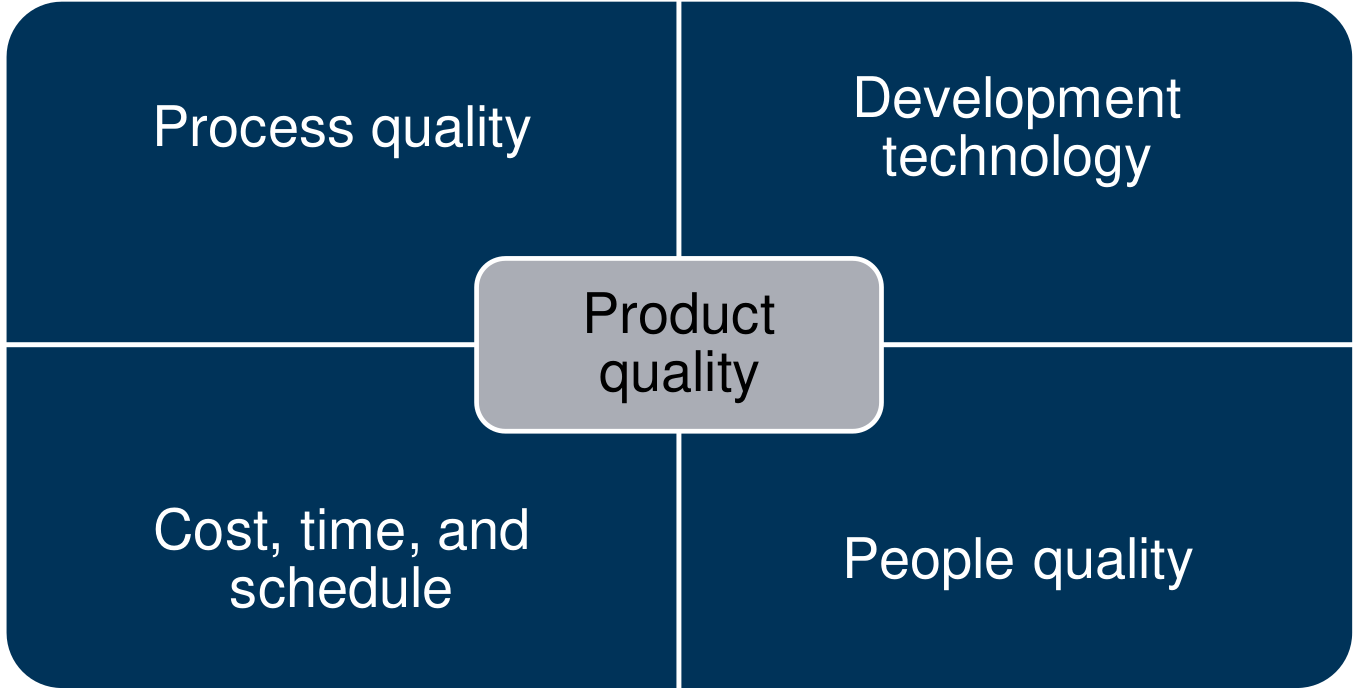
\includegraphics[width=0.5\linewidth]{images/process_vs_quality.png}
    \caption{Correlation between software process and quality}\label{fig:se_process_vs_quality}
\end{figure}

\paragraph{ISO 9000 and 9001}
This is an international set of standards for quality management and applicable to a range of organization branches.
If an organization is to be ISO 9001 conformant, it must document how its
processes relate to the nine core processes:\\

\begin{minipage}[t]{0.49\textwidth}
    \textbf{Product delivery process}
    \begin{itemize}[topsep=0pt, itemsep=0pt]
        \item Business acquisition
        \item Design and Development
        \item Test
        \item Production and delivery
        \item Service and support
    \end{itemize}
\end{minipage}
\begin{minipage}[t]{0.49\textwidth}
    \textbf{Supporting processes}
    \begin{itemize}[topsep=0pt, itemsep=0pt]
        \item Business management
        \item Supplier management
        \item Inventory management
        \item Configuration management
    \end{itemize}
\end{minipage}
\newline

ISO 9001 certification does not imply better quality compared to not certificated software.
The standard only focuses on ensuring that the organization has quality management procedures in place and it follows these procedures.

\begin{figure}[h]
    \centering
    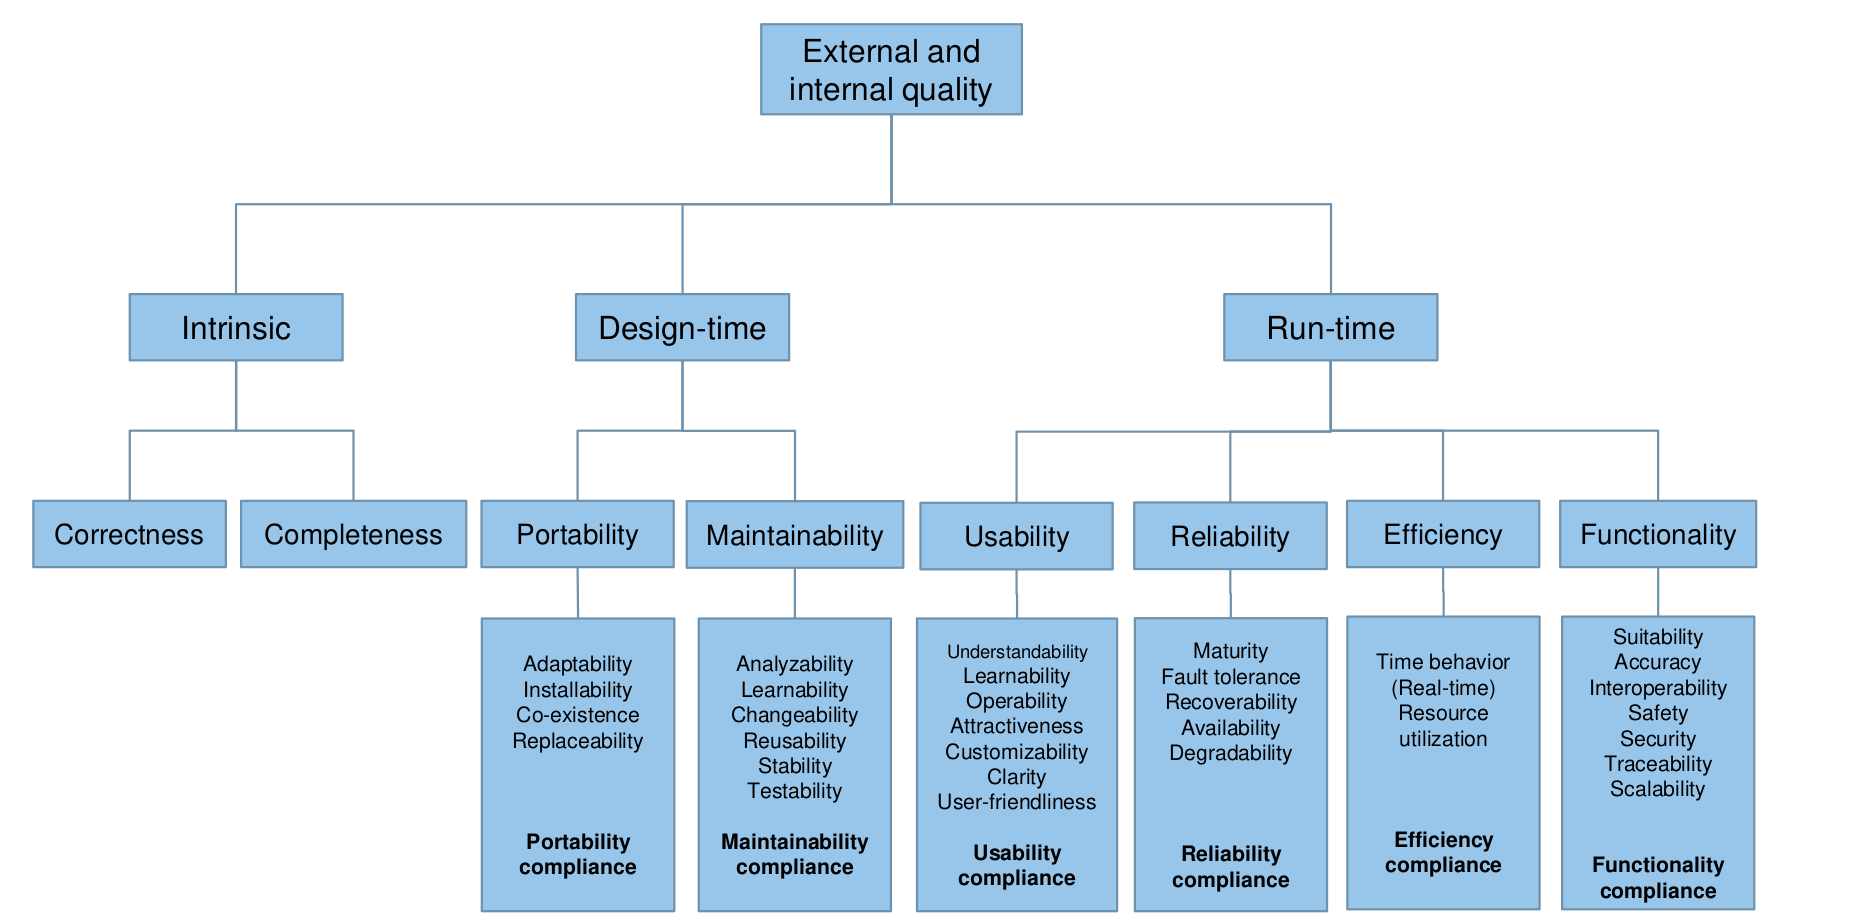
\includegraphics[width=\linewidth]{images/types_of_quality.png}
    \caption{Types of Quality}\label{fig:se_types_of_quality}
\end{figure}
\newpage

%!TEX root = ../summary.tex

\section{From Requirements to System Design}
\subsection{Software Architecture}
Software Architecture is the fundamental organization of a system embodied in its components, their relationships to each other and the environment and the principles guiding its design and evolution.
Its main purposes are quality, the efficiency of the development process, risk minimization, and managing communication and knowledge.\\
Figure~\ref{fig:software_intensive_system_architecture} describes a model of how architecture looks like in software intensive systems.
\begin{figure}[h]
  \centering
  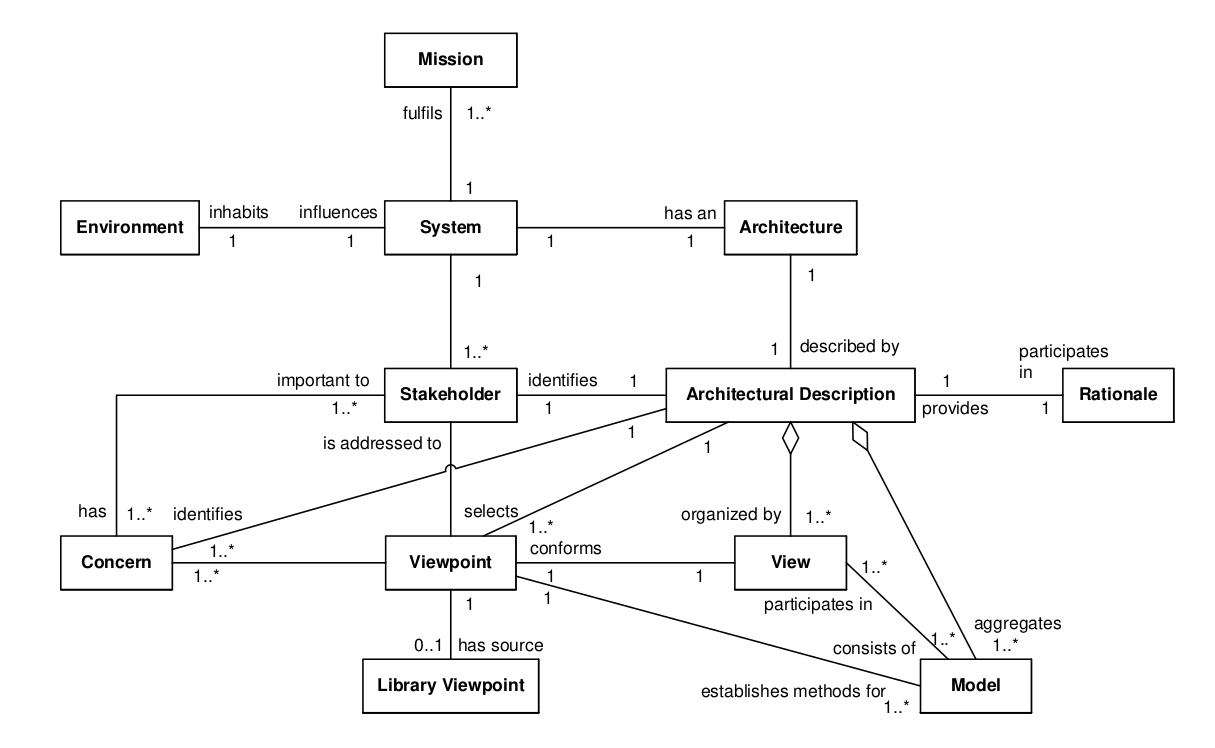
\includegraphics[width=.8\textwidth]{images/software_intensive_system_architecture.png}
  \caption{Architecture in Software Intensive Systems}\label{fig:software_intensive_system_architecture}
\end{figure}

\begin{itemize}
  \item The \textbf{system} is a collection of components which are organized to accomplish a function and has defined boundaries, consists of components and interfaces interacts with its environment through these interfaces and is defined by its static structure and dynamic behavior.
  \item The \textbf{environment} are the developmental, operational, political and other influences on the system.
  \item Every system has an \textbf{architecture} that can be described by an \textbf{architectural description}.
  \item \textbf{Stakeholders} are people that have an interest in the system which can have various roles regarding the architectural description.
  \item \textbf{Concerns} are interests which influence the system's development, its operation or any other aspect that is important to stakeholders.
  \item \textbf{Views} address one or more concerns of the system stakeholders.
  \item A \textbf{viewpoint} then describes a view and any associated modeling methods or analysis techniques by determining the languages for the architectural description
  \item \textbf{(System) models} provide abstractions in different ways.
    The object model describes the structure of the system, the functional model what the system's functions are and a dynamic model how the system reacts to external events.
\end{itemize}

\subsubsection{Modelling}
Models \textbf{reduce} the reality to a subpart of the original where irrelevant parts to the application are omitted which increases abstraction.
This reduction always has a \textbf{purpose} in mind which makes id adequate for a purpose or not and it is always possible to find a \textbf{mappging} between reality and the model.\\
The process of modelling can be divided in the following repeating sub-processes:
\begin{itemize}
  \item \textbf{Understanding} the application domain and its problems and possible solutions
  \item \textbf{Conceptualize} the part of the domain that is of relevance with the help of a concept language
  \item \textbf{Abstract} by outlining the main problems that have to be supported by the system on the basis of forgetful mappings.
  \item \textbf{Define} the main concepts/annotations used for the development of the model.
  \item \textbf{Construct} a model by organizing and linking ideas, judgements or concepts.
  \item \textbf{Evaluate} the model or parts of it considering pre-defined quality characteristics.
  \item \textbf{Refine} with iterative development to make the model more elaborated while maintaining its main structure.
\end{itemize}

\subsubsection{Modularity}
Modularity is the decomposition of a system into components to manage complexity by hiding unnecessary information to the outside world in these components.
This increases maintainability and reusability since the single components can be switched out or used elsewhere.
Also work can be easily distributed to the single components.\\
Functional decomposition decomposes the system regarding functions which implies that one has to understand the whole system to make a change possibly.
A better approach is modular decomposition where modules are the main concepts in a system.
This assumes we can find concepts in a new (greenfield engineering) or existing (reeingineering) software system  and that we can create a component-based interface on any system (interface engineering).\\
When looking at modules, we can either assume a black-box view where we only look at the possible input-output combinations and not the internals of the system or a whit-box view where the internals are regarded.

\subsubsection{Component-based Software Engineering (CBSE)}
CBSE is an approach to software development that relies on the reuse of software components which are a set of classes that can be considered a stand-alone service provider.
Components then interact with each other over published, clear defined and standardized interfaces and are integrated with the help of some middleware.\\
A software component has the following properties:
\begin{itemize}
  \item \textbf{Standardized}: Conformation to a standard component model
  \item \textbf{Independent}: Deployable without dependences to other components or if needed it should be stated in a ``requires'' interface specification.
  \item \textbf{Composable}: All interactions have to happen through the public interface
  \item \textbf{Deployable}: Ability to operate as stand-alone entity on a component platform that provides an implementation of the component. This usually means that binaries are provided so that no compilation is necessary before deployment.
  \item \textbf{Documented}: Syntax and also ideally semantics should be specified
\end{itemize}

Component interfaces are defined as shown in Figure~\ref{fig:component_interfaces}.\\
\begin{figure}[h]
  \centering
  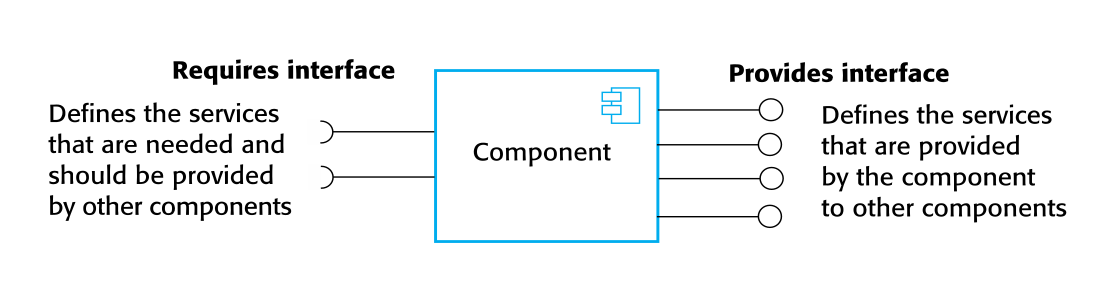
\includegraphics[width=.8\textwidth]{images/component_interfaces.png}
  \caption{Component Interfaces}\label{fig:component_interfaces}
\end{figure}

A component model is a definition of standards for component implementation, documentation and deployment as shown in Figure~\ref{fig:component_model}.
\begin{figure}[h]
  \centering
  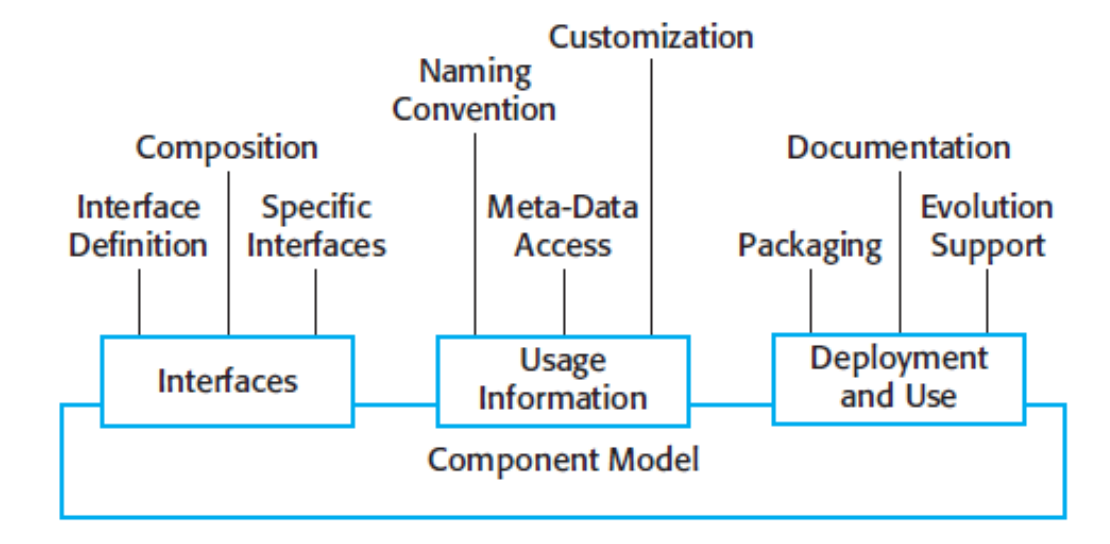
\includegraphics[width=.8\textwidth]{images/component_model.png}
  \caption{Component Model}\label{fig:component_model}
\end{figure}
It specifies how and in which language the interfaces should be defined and the elements which should be included (e.g.\ names, parameters,\ldots).
Furthermore naming conventions are defined for the usage of the component, e.g.\ URIs and meta-data is provided which gives information about interfaces, attributes and helps users to find out what services are provided and required.
Lastly the component model specifies how components should be packaged for deployment usually including all dependencies not specified in the ``required'' interface.\\

After the modelling of the components, they can be composed as shown in Figure~\ref{fig:component_composition}.
\newline

\begin{figure}[h]
  \centering
  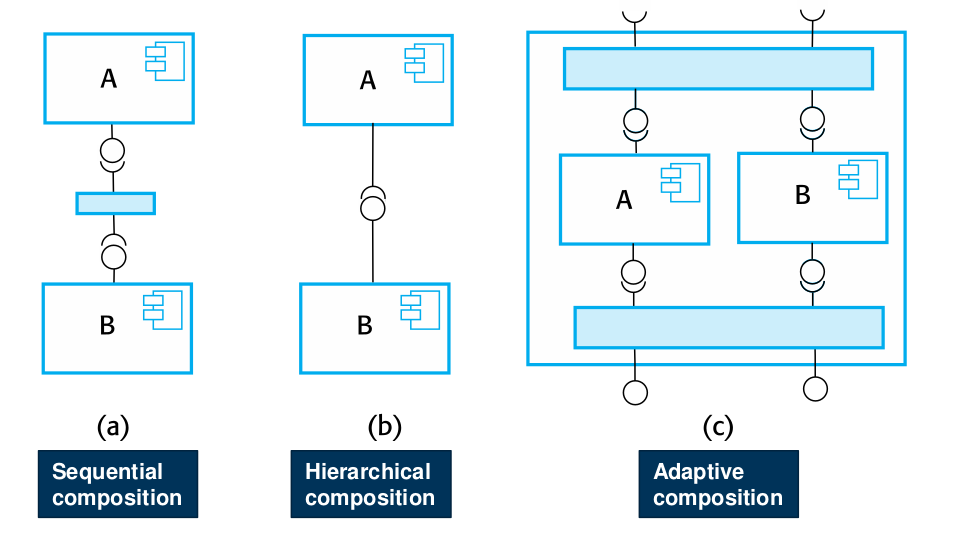
\includegraphics[width=.7\textwidth]{images/component_composition.png}
  \caption{Component Composition}\label{fig:component_composition}
\end{figure}

\begin{minipage}[t]{0.49\textwidth}
    \textbf{Pros}
    \begin{itemize}[topsep=0pt, itemsep=0pt]
        \item Independent components
        \item Component standards to facilitate integration
        \item Middleware to provide support for inter-operability
        \item Development process that is geared to reuse
    \end{itemize}
\end{minipage}
\begin{minipage}[t]{0.49\textwidth}
    \textbf{Cons}
    \begin{itemize}[topsep=0pt, itemsep=0pt]
        \item Component trustworthiness
        \item Component quality certification
        \item Emergent property prediction
        \item Requirements trade-offs (difficult analysis between features of two components)
    \end{itemize}
\end{minipage}

\subsubsection{Design by contract}
Design by contract presents a set of principles to produce dependable and robust object-oriented software.
Thereby a contract is an agreement between the client and the supplier.
Each party expects benefits from the contract and is prepared to incur some obligations to obtain them.
These benefits and obligations are documented in the contract where no obligations than the ones documented can be imposed to a party to obtain the benefits (no hidden clause rule).\\
The design principles design by contract proposes are
\begin{itemize}
  \item \textbf{Non-redundancy}: no tests of preconditions
  \item \textbf{Reasonable preconditions}: precondition is written in the documentation and can by justified according to that specification
  \item \textbf{Failure principle}: execution of rescue clauses to its and, not leading to a retry instruction, causes the current routine to fail.
  \item \textbf{Disciplined exception handling}: The two possible reactions to an exception are retrying or a failure/organized panic.
  \item \textbf{Exception simplicity} Simple rescue clauses that only bring the object back to a stable state, permitting a possible retry
\end{itemize}

\subsubsection{Dependency Structure Matrix (DSM)}
A DSM is a two-dimensional matrix representing the structural or functional interrelationships of objects, tasks or teams.
Each entry in the matrix indicates that the item on the corresponding column depends on the item on the corresponding row.\\
Partitioning on the matrix describes the transformation so that all dependencies are below the diagonal or within groups (interdependencies) and results in a block triangular matrix form.
To eliminate the groups/interdependencies, the corresponding rows and columns can be grouped to one (c.f.\ Figure~\ref{fig:dsm_grouping}).
\begin{figure}[h]
  \centering
  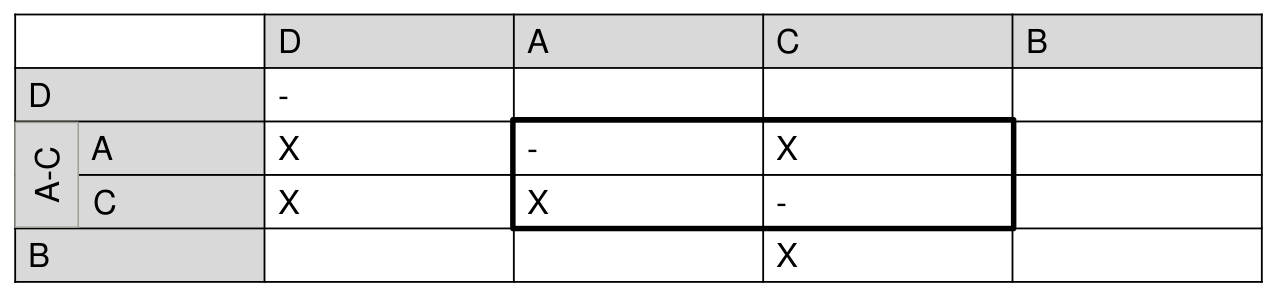
\includegraphics[width=.8\textwidth]{images/dsm_grouping.png}
  \caption{DSM Grouping}\label{fig:dsm_grouping}
\end{figure}

DSMs can be used to identify patterns an anti-patterns in software, c.f.\ Figure~\ref{fig:dsm_layered_pattern} and Figure~\ref{fig:dsm_propagator_anti_pattern}.

\begin{figure}
  \centering
  \begin{minipage}{0.49\textwidth}
    \centering
    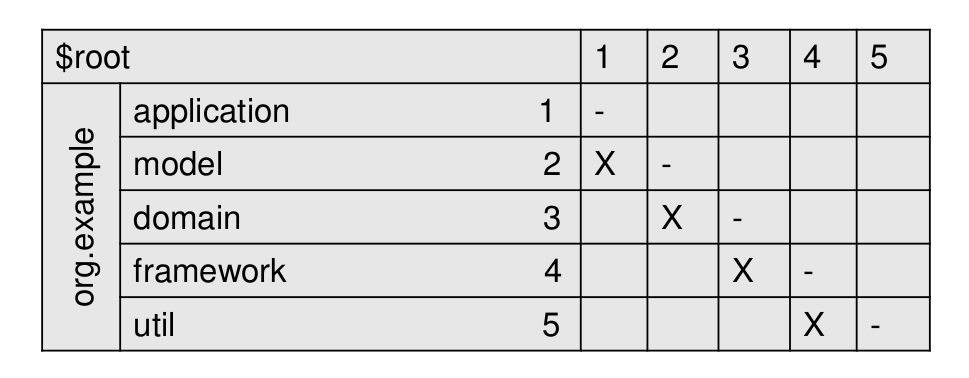
\includegraphics[width=\textwidth]{images/dsm_layered_pattern.png}
    \captionof{figure}{Layered Pattern in DSM}\label{fig:dsm_layered_pattern}
  \end{minipage}%
  \begin{minipage}{0.49\textwidth}
    \centering
    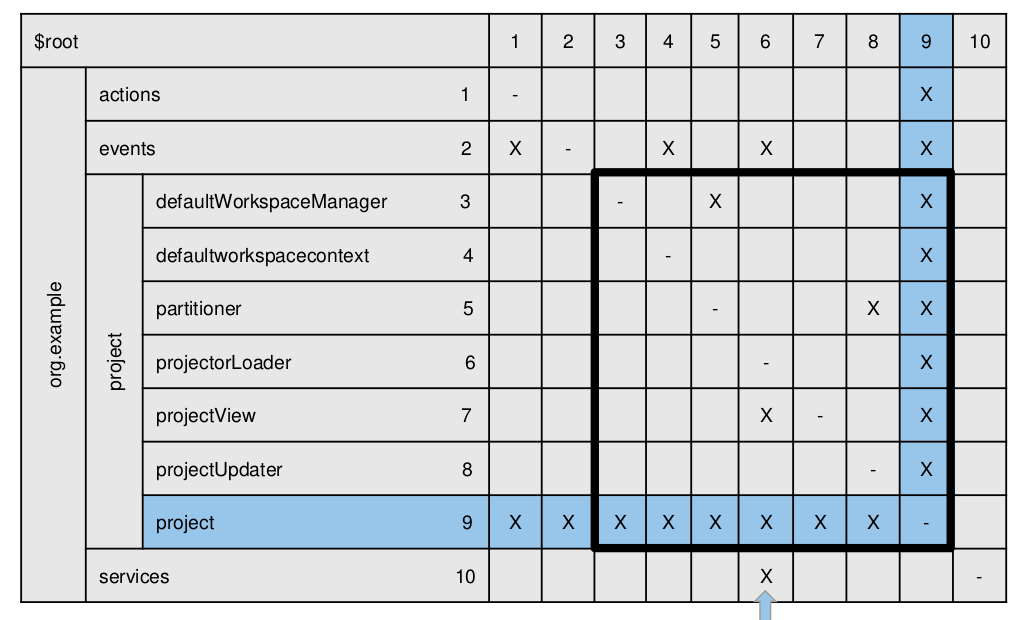
\includegraphics[width=\textwidth]{images/dsm_propagator_anti_pattern}
    \captionof{figure}{Propagator Anti-Pattern in DSM}\label{fig:dsm_propagator_anti_pattern}
  \end{minipage}
\end{figure}

\begin{minipage}[t]{0.49\textwidth}
    \textbf{Pros}
    \begin{itemize}[topsep=0pt, itemsep=0pt]
      \item Better scaling than box-and-line diagrams
      \item Better understanding of information flows
      \item Automatic partitioning algorithms
      \item Efficient cycle detection
      \item Integration of dependency rules
    \end{itemize}
\end{minipage}
\begin{minipage}[t]{0.49\textwidth}
    \textbf{Cons}
    \begin{itemize}[topsep=0pt, itemsep=0pt]
      \item Only as good as the knowledge that goes in (unknown dependencies might exist)
      \item less intuitive than a graph
    \end{itemize}
\end{minipage}

\subsubsection{Guidelines for Modular Design}
\paragraph{Low Coupling and High Cohesion}
We denote the structure of a system as $S = (C,I,CON)$ where C are the components, $env \in C$ the environment, I the interfaces and $CON \subseteq I x I$ is the connection between interfaces.
Figure~\ref{fig:system_structure_notation} shows the notation and possible relationships between components.
\begin{figure}[h]
  \centering
  \begin{subfigure}{.3\textwidth}
    \centering
    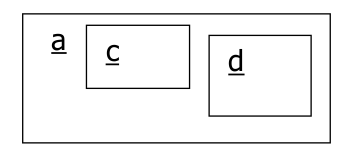
\includegraphics[width=\textwidth]{images/component_parent_relationship.png}
    \caption{Parent relationship\\ $parent(c) = parent(d) = a$\\ $parent(a) = env$}
  \end{subfigure}
  \hspace{.03\textwidth}
  \begin{subfigure}{.3\textwidth}
    \centering
    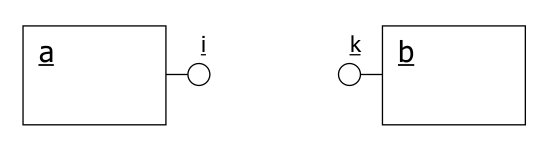
\includegraphics[width=\textwidth]{images/component_interface_relationship.png}
    \caption{Interface-Component Relationship\\ $assigned(i) = a$\\ $assigned(k) = b$}
  \end{subfigure}
  \hspace{.03\textwidth}
  \begin{subfigure}{.3\textwidth}
    \centering
    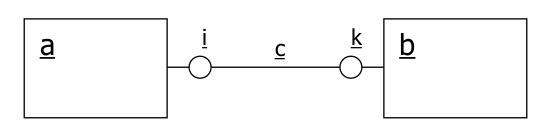
\includegraphics[width=\textwidth]{images/component_connection.png}
    \caption{Connection between Interfaces\\ $connected(c) = (i,k)$}
  \end{subfigure}
  \caption{System Structure Notation}\label{fig:system_structure_notation}
\end{figure}

We then define \textbf{coupling} as the normalized number of connections between components at the same hierarchical level 
\begin{equation*}
  coupling(s) = \frac{|\{con \in s.CON| \exists s,I: con = connected(i,j) \wedge parent(assigned(i)) = parent(assigned(i))\}|}{|s.C|}.
\end{equation*}
The goal is to make coupling as low as possible.

We can define different classes of coupling, in the following listed in decreasing amount of coupling order:
\begin{itemize}
  \item \textbf{Content Coupling}: One component changes another component's data or when control is passed from one component to the middle of another.
  \item \textbf{Common Coupling}: Two components share data which shows a lack of clear responsibility and reduces readability, maintainability and reusability
  \item \textbf{External Coupling}: Components communicate through an external medium such as a file, device interface, protocol or data format.
  \item \textbf{Control Coupling}: One Component directs exaction of another component by passing the necessary control information. This approach can be good if parameters allows factoring and reuse of functionality or bad if parameters indicate completely different behavior or components are not independent.
  \item \textbf{Stamp Coupling}: Complete data structures are passed from one component to another.
  \item \textbf{Data Coupling}: Component passes data (not data structures) to another component.
\end{itemize}

\textbf{Cohesion} is defined as how closely related different responsibilities of a component are. The goal is to make cohesion as high as possible.\\
Like for coupling, we can again define types of cohesion, also in decreasing order:
\begin{itemize}
  \item \textbf{Functional Cohesion}: Every essential element to a computation is contained in the component so that a single input is transformed to a single output. Ideal kind of cohesion in that it maximizes reusability, testability, understandability, learnability, extensibility and maintainability.
  \item \textbf{Sequential Cohesion}: The output of one component is the input of another and data flows between parts. Quite good kind of cohesion.
  \item \textbf{Communicational Cohesion}: Elements operate on the same data
  \item \textbf{Procedural Cohesion}: Elements are related only to ensure a particular order of execution. Actions are weakly connected and unlikely to be reusable
  \item \textbf{Temporal Cohesion}: Elements are independent but are activated around the same point in time. Code is spread out which results in bad maintainability and reusability
  \item \textbf{Logical Cohesion}: Elements are logically related, not functional
  \item \textbf{Coincidental Cohesion}: Elements have no significant relation to each other (worst kind).
\end{itemize}

\paragraph{Single Responsibility Principle}
Every class should only have one responsibility, if there are multiple split the class.
A guideline for this is ``there should never be more than one reason to change a class''.

\paragraph{Separation of Concerns}
Separate features to different components which encapsulate a semantic concern what helps humans to handle complexity (only able to hold around 7 things in mind).
This also enables components to be easily replaced.
Modules therefore designed with the \textbf{open/closed principle} in mind.
This means that a module is open for extension but closed for modification so that the behavior cannot be changed but only extended and thus no unexpected effects will arise.

\paragraph{Liskov Substitution Principle (LSP)}
\begin{chapquote}{Barbara Liskov. (1987)}
    Let $q(x)$ be a property provable about objects x of type T. Then $q(y)$ should
be provable for objects y of type S where S is a subtype of T.
\end{chapquote}
This means child classes should never violate the invariants of the base class or remove some of its behavior.

\paragraph{Interface-Segregation Principle}
Prefer small, cohesive interfaces over big ones.

\paragraph{Anticipate change}
Build components in a way that minimizes effort for potential future changes by finding a compromise between generality and specificity.
A good guideline here is the principle of low coupling and high cohesion.
It is easy to overdo it though, since reusability is oftentimes very difficult.

\paragraph{Do not Repeat Yourself}
Every piece of knowledge (and functionality) must have a single, unambiguous, authoritative representation within a system.
This dramatically improves maintainability.\\
Duplication can either be imposed (developers have no choice due to environment), inadvertent (duplication not realized by devs), due to impatience or lazyness or due to inter-developer communication or the lack thereof.

\subsubsection{Architecture and External Quality}
When introducing a high degree of modularity we influence internal quality by increasing maintainability and reusability.
Testability might be increased or decreased depending on the system though.
External quality might suffer also by introducing to many layers or indirections
which decreases performance and also security might suffer by introducing large attack surfaces.\\

\subsection{Antipatterns}
Antipatterns are commonly occurring solutions to a problem that generates decidedly negative consequences.
They define an industry vocabulary for common defective processes and implementations within organizations.
Antipatterns can concern software development and software architecture.\\
The reasons for these mistakes are called the 7 deadly sins:
\begin{itemize}
  \item Haste
  \item Apathy (not caring)
  \item Narrow-Mindedness (not applying common solutions)
  \item Sloth (solutions based on easy answers)
  \item Avarice (excessive complexity)
  \item Ignorance
  \item Pride
\end{itemize}

Common antipatterns are:
\begin{itemize}
  \item The blob: A ``god class'' that does everything typically caused by the lack of an architecture or the enforcement thereof, too limited intervention or by the specification of the requirements. 
  \item Functional decomposition: Modules are based on functionality instead of semantic parts from the view of the user. It is typically caused by a lack of object-oriented understanding, the lack of architecture enforcement and sometimes due to badly specified requirements
  \item Auto-generated stovepipe: Trying to use the same interfaces of an existing system for a distributed one.
  \item Golden Hammer: Using the same tools for everything
  \item Design by committee: A complex software design is the product of a committee process of too many people. The design is too complex to realize and test due to excessive complexity, ambiguities, over constraint and other specification defects.
\end{itemize}

\subsection{Reuse}
When developing software, it is usually advisable to ``invent the wheel twice''.
Therefor components should be designed with some principles in mind to support reuse:
\begin{itemize}
  \item Modularity to extract and insert modules
  \item Loose coupling high cohesion also to extract modules
  \item Information hiding for plug and play usage
  \item Separation of concerns to be able to tell the responsibilities of a component
\end{itemize}
There are some pitfalls when trying to write reusable components though.
Either technical issues like the reuse is only done at code level which has a very limited scope and is often done unsystematically  or inconsistent or incomplete component specifications reusability or organizational reasons like the lack of planning, motivation or component marketplaces can hinder the development of reusable software.
Also everytime a trade-off between flexibility and stability has to be met so that enough flexibility that reuse is feasible and enough stability to generate benefits is given.\\
Reusable components can either be a side product of development (opportunistic or ad-hoc reuse) or be planned (planned or structured reuse).
Ad-hoc reuse usually dues not scale due the lack of infrastructure to maintain components like search, evaluation, adaption or integration services.
So the better approach is structured reuse where essential functionality is parameterized so that it can easily be customized usually during deployment.\\

\subsubsection{Variability}
Variability can either be visible to the user (external variability) or hidden from them (internal variability).
It is supported by the concept of managed variability which implies defining variability, managing variable artifacts, supporting activities concerned with resolving variability and collecting, storing and managing trace information necessary to fulfill these tasks.
The time when variabilities are resolved is called binding time.\\
Defining variability can be done as an integral part of development artifacts, which increases their complexity though, or in a separate model.

\paragraph{Orthogonal Variability}
An orthogonal variability model is a model that defines the variability of a software product line. It relates the variability defined to other software development models such as feature model, use case models, design models, component models, and test models.\\

On requirement level, variability is modeled as feature diagram where parts can be mandatory or optional and have interdependencies.
A variation point is defined as a representation of a variability subject and a variant then is a representation of a variability point.
Figure~\ref{fig:feature_diagram} shows an example of a feature diagram.\\
\begin{figure}[h]
  \centering
  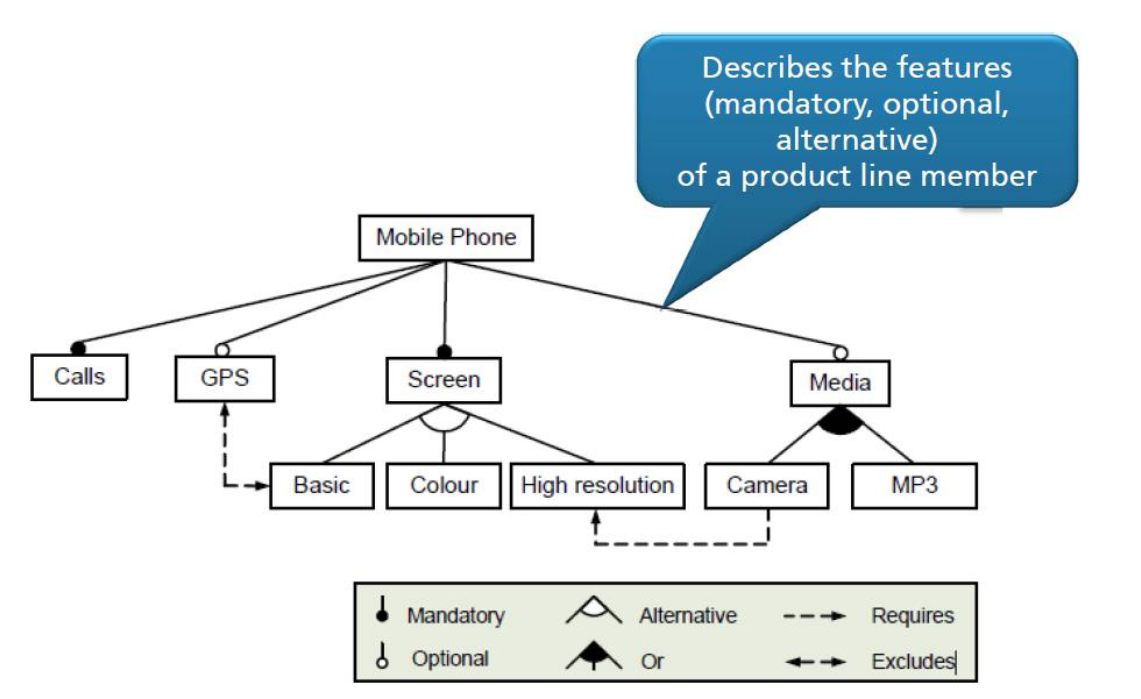
\includegraphics[width=.8\textwidth]{images/feature_diagram.png}
  \caption{Feature Diagram}\label{fig:feature_diagram}
\end{figure}

On code level, variety can be supported with conditional compilation, polymorphism, frame technology or aspect-oriented programming.

\subsubsection{Product Line Engineering (PLE)}
A software product line is a set of applications with a common architecture and shared components, with each application specialized to reflect different requirements.
Specialization can take place in several domains including platform, environment, functions and processes.\\
PLE then is the process of developing a product line with a heavy focus on reusability by separating development into \textbf{family engineering} and \textbf{application engineering}.
Figure~\ref{fig:product_line_engineering} shows an illustration of this process.
\begin{figure}[h]
  \centering
  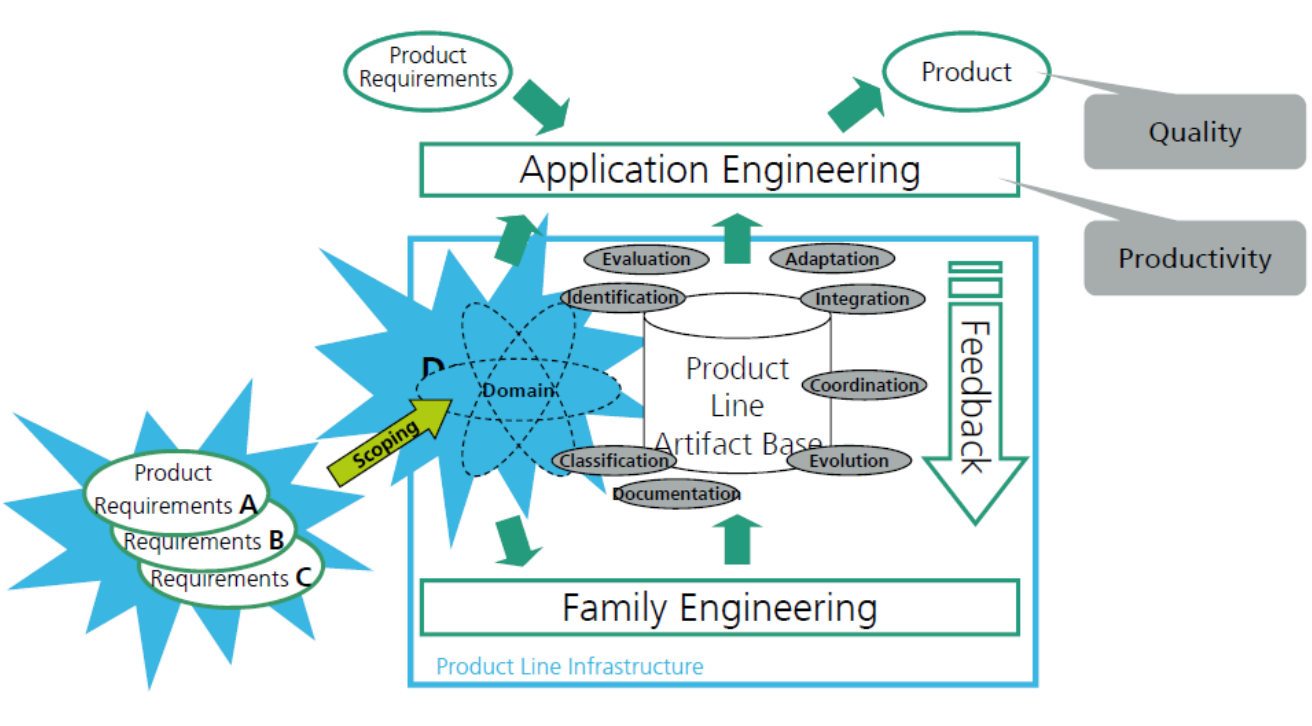
\includegraphics[width=.7\textwidth]{images/product_line_engineering.png}
  \caption{Product Line Engineering}\label{fig:product_line_engineering}
\end{figure}
In family or domain engineering product commonalities and variabilities are identified and reusable (product line) artifacts are developed.
An essential part of this is the scoping of the product line by defining sharp boundaries based on most of the concrete product requirements (all is not economical most of the time).
Important aspects of this are which products will be in the line, which domains to consider, which features are required and which assets are in the line.
These base artifacts cover variability as well as commonalities of the PL and are stored in the \textbf{product line artifact base}.
During the application engineering process their variabilities then are instantiated according to the specific product requirements and thus individual products are developed.\\

\begin{minipage}[t]{0.49\textwidth}
    \textbf{Pros of well-done PLE}
    \begin{itemize}[topsep=0pt, itemsep=0pt]
        \item Reduces development costs
        \item Increases quality
        \item Decreases time-to-market
        \item Better understanding of the domain
        \item Structured reuse possible
    \end{itemize}
\end{minipage}
\begin{minipage}[t]{0.49\textwidth}
    \textbf{Cons}
    \begin{itemize}[topsep=0pt, itemsep=0pt]
        \item High up-front invenstments
        \item Strong domain knowledge and therefore experts necessary
        \item May result in a badly scoped domain what leads to unwanted assets
        \item Limited success in reality
    \end{itemize}
\end{minipage}

\subsubsection{Reference Architectures and Frameworks}
\paragraph{Software Frameworks}
A framework is a set of classes that embodies an abstract design for solutions to a family of related problems, and supports reuse at a larger granularity than classes.
Frameworks support design reuse by providing a skeleton architecture for the application as well as the reuse of specific classes and are language specific.
Applications using a framework extend generic classes of the framework in so called extension points or hot-spots.\\
The main difference to a library is the call hierarchy.
Frameworks call the application specific classes whereas when using a library the application calls the library code.
Also frameworks usually already provide a semi-complete application whereas libraries are only pluggable parts of it.

\paragraph{Reference Architectures}
A Reference architecture is an abstract software architecture for a specific application area. It defines structures and types of software elements, and their interactions and responsibilities. The defined structures are applicable for all systems of a domain.
There are three different types of reference architectures described in Figure~\ref{fig:reference_architectures}.
\begin{figure}[h]
  \centering
  \begin{tabular}{|p{.225\textwidth}|p{.225\textwidth}|p{.225\textwidth}|p{.225\textwidth}|}
    \hline
    & Functional & Logical & Technical\\
    \hline
    Phase of the development process & Requirements analysis & Conceptual design & Detailed design, Implementation\\
    \hline
    Provides a basis for & Functional specification, planning of subsystems & Logical architecture, planning of the implementation & Detailed architecture, implementation, deployment\\
    \hline
    Elements & Functional areas as units of functionality & Components as units of design and implementation & Components as units of implementation and deployment\\
    \hline
    Stakeholder & User, manager, project leaders & Project leaders, architects, developers & Architects, developer, maintenance staff\\
    \hline
    Architectural overview & Functional areas, data flow & Components, layers to be implemented & Technical components, layers which can be deployed\\
    \hline
    Textures (structures, principles and design concepts which occur often) & - & Design rule, may be expressed as a design pattern & Design rule, design pattern, code template\\
    \hline
    Reference interfaces & Named interfaces, if any & Named interfaces; defined in an implementation neutral definition language (e.g., IDL), if necessary & Defined in the programming language used\\
    \hline
    Infrastructure & - & Basic properties & Exactly defined\\
    \hline
  \end{tabular}
  \caption{Types and Elements of a reference architecture}\label{fig:reference_architectures}
\end{figure}

\subsection{Testability}
In general testing or the assessment thereof is a very difficult topic to approach since we often do not know what metrics apply for good tests or tests suits and oftentimes that depends on the system under test.\\
For that reason it is also quite difficult to measure the testability of a system, nevertheless we will try to give some definitions.
All testing theory is mostly academic though, despite having a big importance in industry as well.\\

The first approach defines testability as the degree to which a system or component facilitates the establishment of test criteria and the performance of tests to determine whether those criteria have been met.\\

The second one tries to cast the problem to one of information loss which occurs if the input values to a program do not propagate to the output.
This might happen implicitly if many input values yield the same output or explicitly if local variables are not checked after execution.
With this in mind, we then define testability as the domain/range ration $DRR = \frac{|input~domain|}{|output~domain|}$.
If the DRR is large, testability is poor.
In case of implicit losses, we cannot do much since this depends on the specification.
If we have explicit losses, one solution might be to increase the observability by increasing the size of the output domain by explicit observations.
We might also increase the controllability for being able to also change modules internal states.
By increasing observability and controllability, we need information about who modules work which contradicts the ideas of modularity, encapsulation and information hiding though.\\

A last approach then would be to define testability as likelihood of a program to fail with the next test (given a particular assumed input distribution) if the software includes a bug.
Although this might be a better definition for the quality of tests.
With that definition we can try to inject defects into our programm and see if the output changes.
By measuring the likelihood of such a change we can define that as the amount of testability our program has.

\subsection{Safety}
Systems, no matter in what domain, are usually never to 100\% safe in reality.
Therefore we define a safe system as a system that is above a specified safety threshold.
So the goal is to determine how safe is safe enough without over- or under-engineering a product.

\subsubsection*{Risk}
Before we define such a threshold though, we have to define a measurement scale.
For that we will use risk what is defined as the probability of the occurrence of harm times the severity $R = PHarm \cdot SHarm$ and harm as the physical damage to persons or the environment according to IEC 61508 and ISO 26262 (fundamental security standards).\\
What is to note here that risk perception does usually not represent the actual risk.
Risk perception is the subjective judgement that people make about the characteristics and severity of a risk.
Risk aversion then is the reluctance of people to accept a bargain with an uncertain payoff rather than another bargain with more certain, but possibly lower, expected payoff and scale aversion then is the tendency to want greater protection where consequences are high.\\

In reality risk is usually reduced to a level where it is \textbf{as low as is reasonable practical (ALARP principle)}.
This reduction can take place in several aspects of systems: external measures like guardrails besides roads, electronics and software and other technologies like hydraulic back-ups.
The process of risk reduction is depicted in Figure~\ref{fig:risk_reduction_process}.\\
\begin{figure}[h]
  \centering
  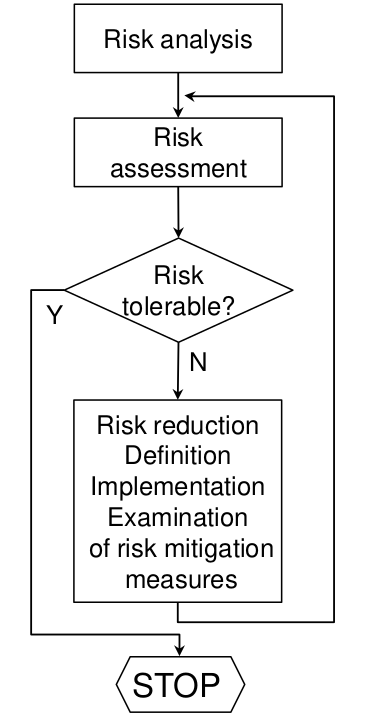
\includegraphics[width=.8\textwidth]{images/risk_reduction_process.png}
  \caption{Risk Reduction Process}\label{fig:risk_reduction_process}
\end{figure}

With these definitions in mind we can define safety as freedom or absence of unacceptable or unreasonable risk (complies to IEC and ISO).

\subsubsection*{Faults, Errors and Failures}
\begin{figure}[H]
  \centering
  
\includegraphics[width=.8\textwidth]{images/fault_error_failure.png}
\end{figure}
A fault is an abnormal condition that can cause an element or an item to fail.
An error is defined as the discrepancy between a computed, observed or measured value or condition and the true, specified or theoretically correct value or condition and a failure then is the actual termination of the ability of an element to perform a function as required.

Faults will lead to errors but errors not necessarily to failures due to error correction and redundancy.\\
Causes of faults can be random issues like damage of fatigue or systematic issues like specification or design problems.
Random failures can only occur in hardware and can be predicted with reasonable accuracy whereas systematic failures can be in hardware or software and can only be eliminated by a change in design or manufacturing and cannot be predicted.
Latter ones can be tried to be avoided during the design and production phase by using techniques and procedures that aim to avoid the introduction of faults.
Furthermore tolerance during operation can be introduced as mentioned before.
This introduction of tolerance can also be applied for random faults.\\

Failures of components can cause faults in systems which result in errors and maybe failures of the system.
This can happen in a cascading fashion where component A fails, afterwards component B, \ldots until the system fails.
Another way for system failure is a common cause failure where one root cause lets several components fail ``simultaneously'' which might ultimately lead to a system failure.

\subsubsection*{Functional Safety}
Functional safety focusses on the hazards (= potential source of harm) and risks originating from the function of an (E/E) system.

The lifecycle approach in this context is an concept from 1947 which defines: The primary concern of the safety life cycle is the management of hazards: their identification, evaluation, elimination, and control through analysis, design and management procedures.
Based on this concept, multiple functional safety standards arose which describe a safety lifecycle and identify activities and requirements based on it.
An example is shown in Figure~\ref{fig:iso26262_software_lifecycle}
\begin{figure}[h]
  \centering
  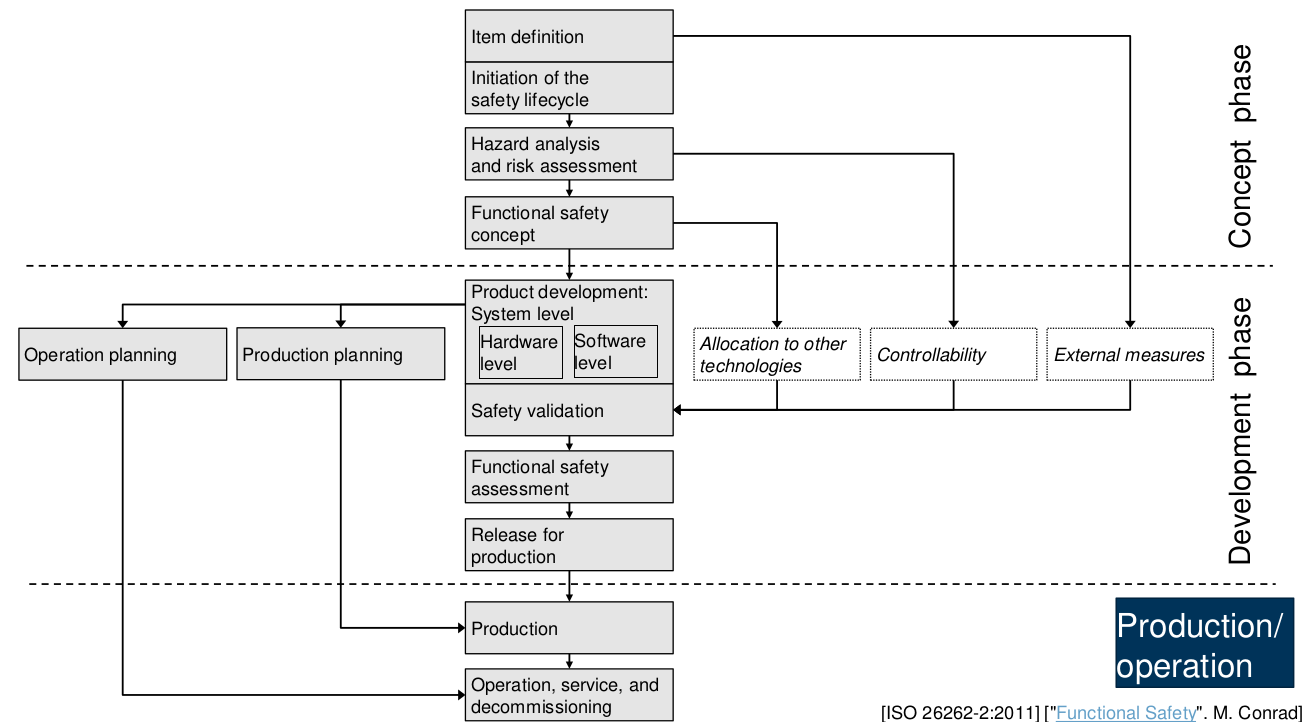
\includegraphics[width=.8\textwidth]{images/iso26262_software_lifecycle.png}
  \caption{ISO 26262 Software Lifecycle Model}\label{fig:iso26262_software_lifecycle}
\end{figure}

\subsubsection*{Safety Analyses using FMEA and FTA}
Safety Analyses examine the consequences of faults and failures of functions, behavior and design of elements and provide information on conditions that could lead to the violation of safety goals.
Furthermore they contribute to the identification of new non-functional hazards not discovered before.
This is done on multiple levels of abstraction during the concept and product development phase.\\
Qualitative analysis methods identify failures and do not predict their frequency whereas the quantitative approach does actually predict the frequency e.g.\ with Markov models.
Another classification differentiates inductive vs deductive methods.
Inductive ones (\textbf{failure mode and effects analysis (FMEA)}) are bottom-up methods which start with root causes to forecast unknown effects whereas deductive analysis methods (\textbf{fault tree analysis (FTA)}) go top-down and try to find out root causes from known effects.
FMEA and FTA approaches are shown in Figures \ref{fig:fmea} and \ref{fig:fta}
\begin{figure}
  \centering
  \begin{minipage}{0.49\textwidth}
    \centering
    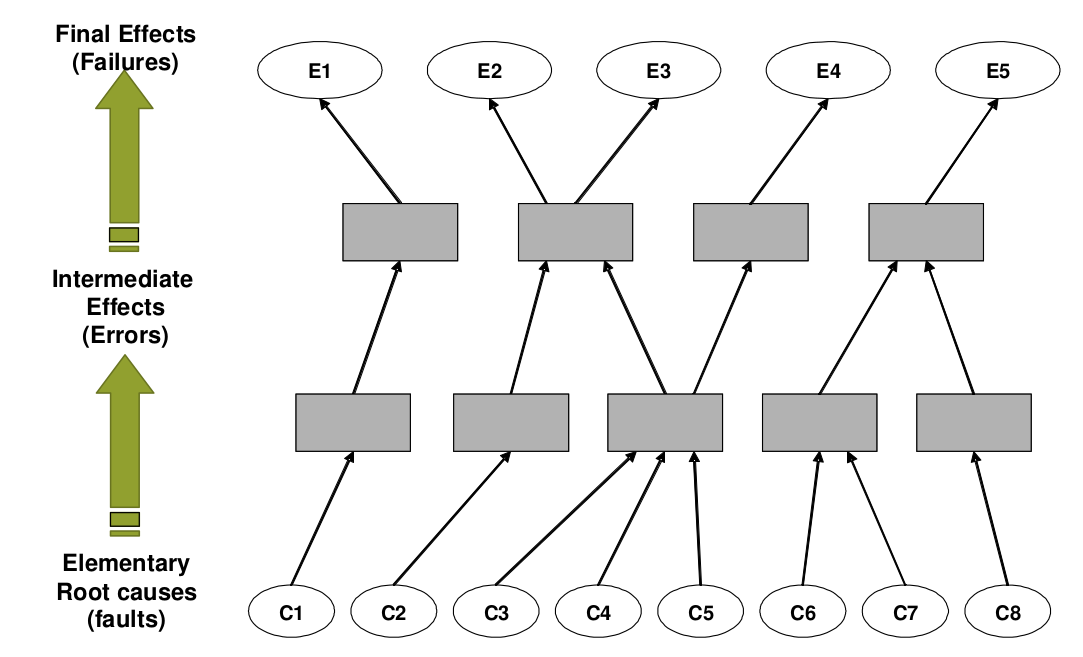
\includegraphics[width=\textwidth]{images/fmea.png}
    \captionof{figure}{Failure Mode and Effect Analysis}\label{fig:fmea}
  \end{minipage}%
  \begin{minipage}{0.49\textwidth}
    \centering
    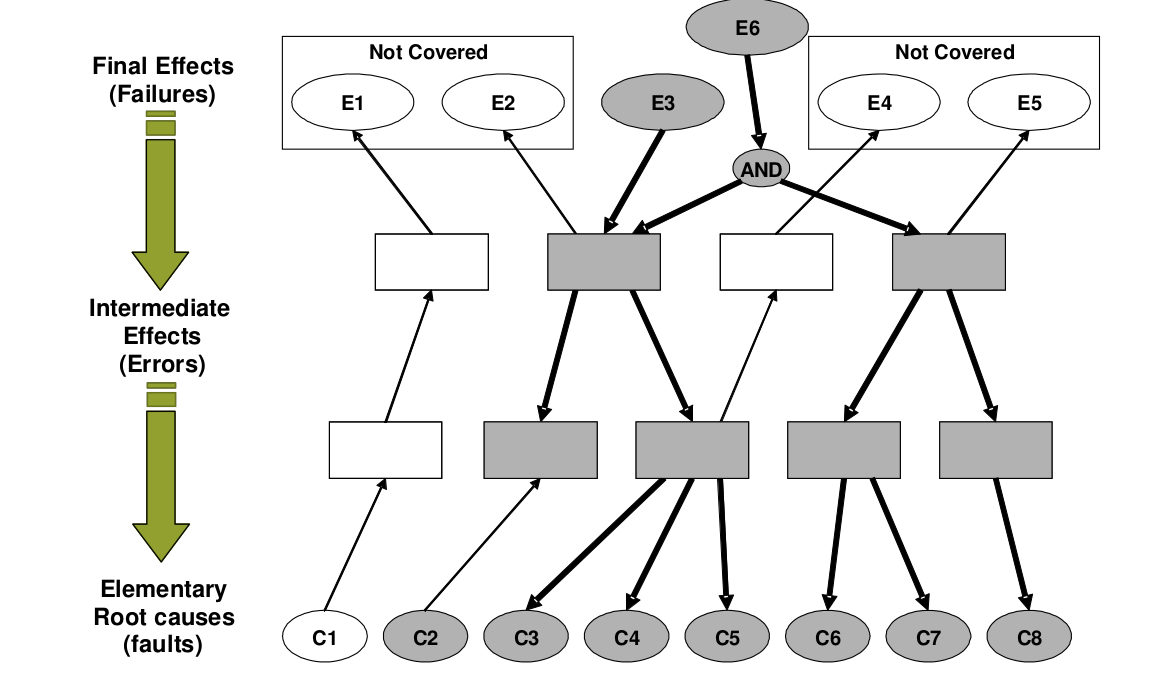
\includegraphics[width=\textwidth]{images/fta.png}
    \captionof{figure}{Fault Tree Analysis}\label{fig:fta}
  \end{minipage}
\end{figure}

\paragraph{Design FMEA}
\begin{figure}[H]
  \centering
  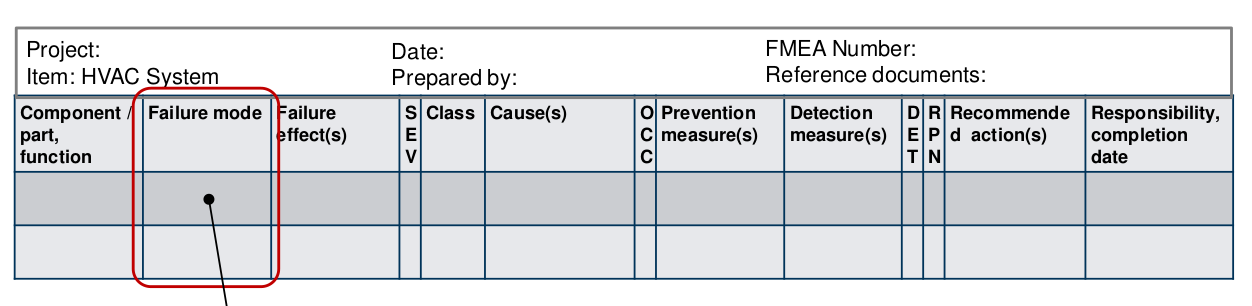
\includegraphics{images/design_fmea.png}
  \caption{Design FMEA}
\end{figure}
\begin{description}
  \item[Failure mode] Manner in which a component might fail to meet design intent
  \item[Failure Effects] Effects of the failure mode on the functions perceived by the customer
  \item[Causes] Indication of the design weakness causing the failure mode
  \item[Detection/Prevention Measures] Activities that assure the design adequacy for the failure
  \item[Severity (SEV)] Severity of potential failure effect on a scale from 1 to 10
  \item[Occurence (OCC)] Likelihood of the failure on a scale from 1 to 10
  \item[Detection (DET)] Likelihood of not detecting the failure before reaching the end-user on a scale from 1 to 10
  \item[Risk Priority Number (RPN)] $RPN = SEV \cdot OCC \cdot DET$ used for priorization of concerns and actions
\end{description}

\paragraph{FTA}
Procedure:
\begin{enumerate}
  \item Plan of the system and FMEA (if existing) as input.
  \item Define system under scrunity
  \item Determine undesired events/failures
  \item Identify event or series of events that lead to top-level event
  \item Apply recursively (apply AND/OR symbols)
  \item Identify cut sets, a set of events that, taken together, lead to system failure.
\end{enumerate}

\newpage

% Needs to be enabled when there are any references.
% \clearpage
% \addcontentsline{toc}{section}{\refname}
% \printbibliography

\end{document}
